\part{Einführung}\label{part:einfuhrung}
\frame{\partpage}

\frame{\frametitle{Einführung}\tableofcontents[part=2, hideallsubsections]}


\section{Notwendigkeit von Forschungssynthesen}


\begin{frame}
  \frametitle{Gründe für die Durchführung einer Forschungssynthese}
  \begin{itemize}[<+->]
  \item Unsicherheit über die Wirksamkeit von Maßnahmen (Interventionen) (Politik, Schule, Medizin etc.).
  \item Fehlender Gesamtüberblick über einen bestimmten (wissenschaftlichen)
    Forschungsbereich, um sinnvoll weitere (methodische wie inhaltliche)
    Forschung zu initiieren.
  \item \ldots
  \end{itemize}
\end{frame}


\begin{frame}
  \frametitle{"Wächst der Wissenschaft das Wissen über den Kopf?"}
  \begin{itemize}
  \item "`But today we are experiencing a crisis of faith; many of us no longer feel sure that science, though growing
    explosively, is moving inexorably toward the truth. [\ldots] increasingly chaotic output of contemporary research"'
    (Hunt 1997: 1).
  \item "`Literaturflut - Informationslawine - Wissensexplosion. Wächst der Wissenschaft das Wissen über den Kopf?"'
    (Marx\,/\,Gramm 2002)
  \item \ldots
  \end{itemize}
\end{frame}


\begin{frame}
  \frametitle{Indikatoren für eine "`Informationslawine"' in den empirischen Sozialwissenschaften}
  \begin{itemize}[<+->]
  \item Das Kölner Zentralarchiv für empirische Sozialforschung erfasst 150 bis 200 Studien p.a. (pers. Kommunikation mit
    Oliver Watteler vom 2. Mai 2008)
  \item 120 Publikationen zum Trennungs-/Ehescheidungsrisiko in Europa (Wagner/Weiß 2006)
  \item17 Publikationen und 20 Originaldatensätze über 24 Städte in NRW zu Wanderungsmotiven (Bleck/Wagner 2006)
  \item 15 Individualdatensätze mit Angaben von \numprint{80000} Jugendlichen zum Schulschwänzen (Weiß 2008)
  \item \ldots
  \end{itemize}
\end{frame}


\begin{frame}[plain]\frametitle{Eingereichte und veröffentlichte Manuskripte in
    der Kölner Zeitschrift für Soziologie und Sozialpsychologie}
  \begin{center}
    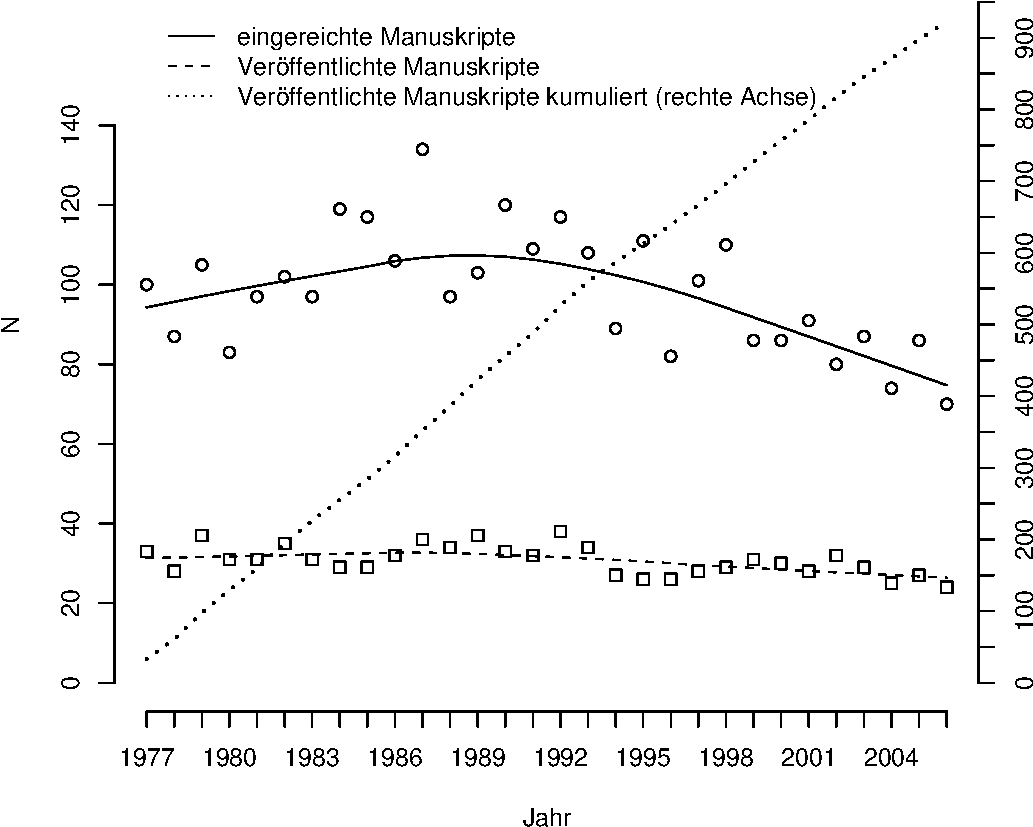
\includegraphics[scale = 0.5]{figKZFSS}
  \end{center}
\end{frame}


\begin{frame}
  \frametitle{Wie lassen sich große Mengen an Forschungsbefunden aufbereiten?}
  %%
  \begin{enumerate}
  \item \textbf{Bibliographien} ("`Fischer, Sonja (Hg.), 2005: Schulmüdigkeit
    und Schulverweigerung. Eine annotierte Bibliografie für die Praxis. München:
    DJI"')
  \item \textbf{Narrative Reviews} ("`Blumel, Susan R., 1992: Explaining Marital
    Success and Failure. S. 1-114 in: Bahr, Stephan J. (Hg.), Family Research. A
    Sixty Year Review, 1930-1990. New York: Lexington Books."')
  \item \textbf{Systematische Reviews\,/\,Forschungssynthesen}
    \begin{itemize}
    \item Qualitative Ausrichtung
    \item Quantitative Ausrichtung (Meta-Analyse)
    \end{itemize}
  \end{enumerate}
\end{frame}


\begin{frame}
  \frametitle{Grenzen von Bibliographien und narrativen (qualitativen) Reviews}
  \begin{itemize}
  \item<+-> Publikationsauswahl ist häufig unsystematisch und intersubjektiv nicht nachvollziehbar (\emph{confirmation bias}).
  \item<+-> Kein/Unzureichender Umgang mit \emph{widersprüchlichen} Befunden.
  \item<+-> Kein/Unzureichender Umgang mit \emph{vielen} empirischen Befunden.
  \item<+-> Ausmaß der Variabilität der Befunde kann nicht bestimmt werden.
  \item<+-> Erklärungen der Variabilität der Befunde können nicht überprüft werden.
  \end{itemize}
\end{frame}



\section{Begriffliche und konzeptionelle Grundlagen}

\begin{frame}<+->\frametitle{Vielfalt an Begriffen}
  %%
  \begin{itemize}
  \item Systematischer Review\,/\,Systematischer Übersichtsartikel
    (\emph{Systematic review})
  \item (Quantitative) Forschungssynthese (\emph{(Quantitative) Research
      synthesis})
  \item Integrativer Review (\emph{Integrative review})
  \item Meta-Analyse, Metaanalyse (\emph{Meta-analysis})
  \end{itemize}
\end{frame}


\begin{frame}
  \frametitle{Systematischer Reviews und Meta-Analysen}
  \begin{block}{Systematic (literature) review}
    "`A review that strives to comprehensively identify, appraise, and
    synthesize all the relevant studies on a given topic. Systematic reviews are
    often used to test just a single hypothesis, or a series of related
    hypothesis."'
  \end{block}
  %%
  \begin{block}{Meta-analysis}
    "`A review that uses a specific statistical technique for synthesizing the
    results of several studies into a single quantitative estimate (i.e. a
    summary effect size)"' \citep[19]{petticrew_systematic_2006}.
  \end{block}
\end{frame}


\begin{frame}\frametitle{Begriff der Meta-Analyse nach Glass (1976) }
  %%
  \enquote{Meta-analysis refers to the analysis of analyses. I use it to refer to the
  statistical analysis of a large collection on analysis results from individual
  studies for the purpose of integrating the findings} \citep[3]{glass_primary_1976}.
\end{frame}


\begin{frame}\frametitle{Begriff der Meta-Analyse nach Drinkmann (1990)}
  %%
  \enquote{Mit Meta-Analyse wird eine an den Kriterien empirischer Forschung
    orientierte Methode zur quantitativen Integration der Ergebnisse empirischer
    Untersuchungen sowie zur Analyse der Variabilität dieser Ergebnisse
    bezeichnet} \citep{drinkmann_methodenkritische_1990}.
\end{frame}


\begin{frame}
  \frametitle{Begriff der Meta-Analyse nach Borenstein et al (2009)}
  "`Meta-analysis refers to the statistical synthesis of results from a series
  of studies. While the statistical procedures used in a meta-analysis can be
  applied to any set of data, the synthesis will be meaningful only if the
  studies have been collected systematically. This could be in the context of a
  systematic review, the process of systematically locating, appraising, and
  then synthesizing data from a larger number of sources."' (Borenstein et
  al. 2009: xxif.)
\end{frame}


\begin{frame}\frametitle{Zum Verhältnis von systematischem Review, Forschungssynthese und Meta-Analyse: Ein Fazit}
  %%
  \begin{itemize}[<+->]
  \item Der Begriff (quantitative) Forschungssynthese (oder: quantitativer
    systematischer Review) beschreibt den gesamten
    Forschungsprozess. Forschungssynthesen haben sowohl \emph{qualitative} als
    auch \emph{quantitative} Elemente.
  \item Der quantitative (statistische) Teil einer Forschungssynthese heißt
    \emph{Meta-Analyse}.
  \end{itemize}
\end{frame}


\begin{frame}\frametitle{Systematik von Meta-Analysen I}
  %%
  \begin{itemize}[<+->]
  \item (Typ I: Qualitative Zusammenfassung, klassisches narratives Review)
  \item Typ II: Quantitative Zusammenfassung von publizierten, aggregierten
    Statistiken ("`publikationsbasierte"' Meta-Analyse)
  \item Typ III: Neuauswertung auf der Basis von zusammengeführten Originaldaten
    ("`originaldatenbasierte"' Meta-Analyse)
  \item Typ IV: Prospektiv geplante, gepoolte Auswertungen
  \end{itemize}
  
\citetext{Quellen: \citealt[149]{blettner_vergleich_1997}, \citealt[91]{finney_statistician_1995}}
\end{frame}


\begin{frame}\frametitle{Systematik von Meta-Analysen II}
  \begin{itemize}[<+->]
  \item Analyseebene: Aggregat- (APD) oder Individualdaten (IPD)
  \item Skalierung der abhängigen Variablen
  \item Forschungsdesign:
    \begin{itemize}
    \item Experiment oder Beobachtung\,/\,Befragung
    \item Intervention oder Zusammenhang
    \end{itemize}

  \end{itemize}
  (Sauerbrei und Blettner 2003)
\end{frame}



\begin{frame}
  \frametitle{Vier prototypische Forschungsprobleme von Forschungssynthesen}
  \begin{itemize*}
  \item<+-> Deskription
    \begin{itemize}
    \item<+-> Verbreitung des Schulschwänzens (Weiß 2008)
    \item<+-> Meta-Analyse von Studien zur Motivation von Stadt-Umland-Wanderung (Bleck/Wagner 2006)
    \end{itemize}
  \item<+-> Exploration: Meta-Analysen zum Stand der Ehescheidungsforschung (Wagner/Weiß 2003; 2004)
  \item<+-> Hypothesentests: Meta-Analysen zum Ehescheidungsrisiko in Europa (Wagner/Weiß 2006)
  \item<+-> Evaluation (von Interventionen): Meta-Analyse zur Wirksamkeit von Psychotherapien (Smith/Glass 1977)
  \end{itemize*}
\end{frame}



\begin{frame}
  \frametitle{Geschichte der Meta-Analyse}
  \begin{itemize}
  \item<+-> Erste Entwicklungen von Pearson (1904), Fisher (1932), Cochrane (1937).
  \item<+-> Zwischen 1930 und 1970 erfolgte keine Weiterentwicklung.
  \item<+-> Mitte der 1970er Jahre neues Forschungsinteresse: Glass (1976) prägt den Begriff "`Meta-Analyse"'
  \item<+-> In den 1980er Jahren bereits fünf Monographien: Glass et al. 1981, Hunter et al. 1982, Rosenthal
    1984, Light/Pillemer 1984, Hedges/Olkin 1985.
  \item<+-> Ab Mitte der 1980er Jahre kontinuierliche Anwendung und
    Weiterentwicklung der Methode in der Psychologie, Pädagogik und Medizin.
  \item<+-> In einigen Fächern bereits voller Institutionalisierungsgrad.
  \end{itemize}
\end{frame}


\begin{frame}\frametitle{Verschiedene Disziplinen kennen verschiedene "`Meta-Analyse-Schulen"'}
  %%
  \begin{itemize}
  \item Psychologie
  \item Erziehungswissenschaften
  \item Medizin, Gesundheitswissenschaften, Epidemiologie
  \item VWL (und BWL)
  \item (Soziologie)
  \end{itemize}
\end{frame}

\begin{frame}[plain]
  \frametitle{Soziologische Forschungssynthesen (SSCI)}
  \begin{center}
    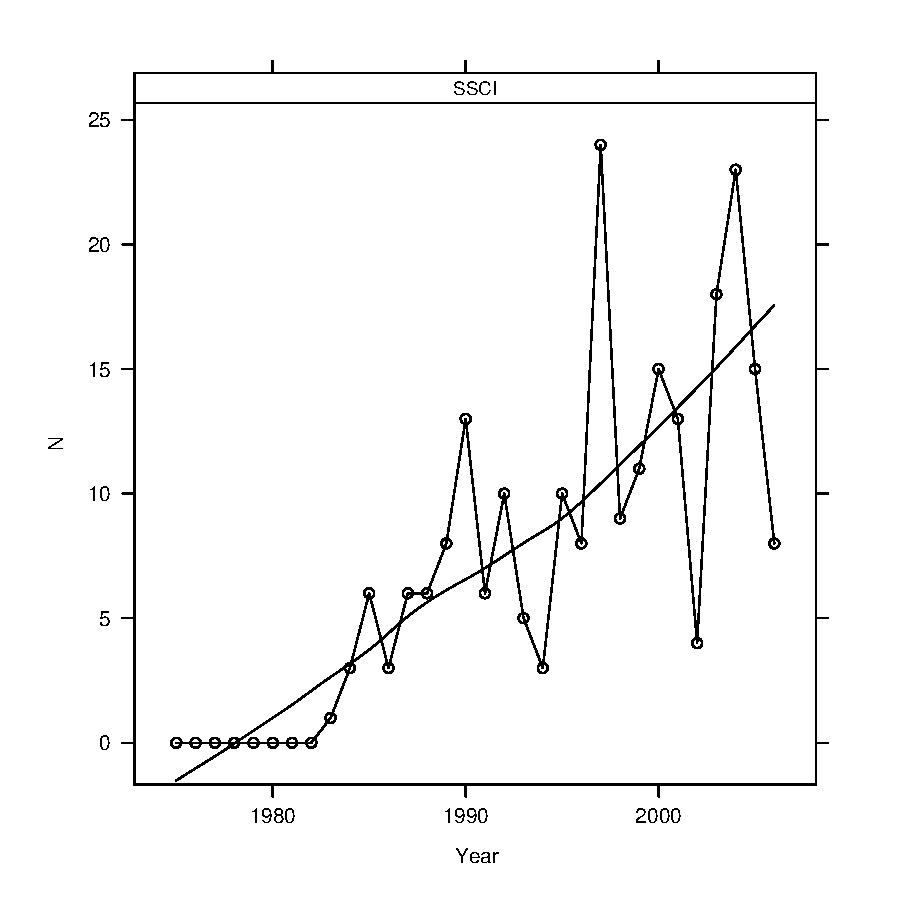
\includegraphics[scale = 0.55]{figLitDB-SSCI}
  \end{center}
\end{frame}





\section{Vorteile von Forschungssynthesen}


\begin{frame}
  \frametitle{Vorteile von (quantitativen) Forschungssynthesen}
  \framesubtitle{Systematisch, strukturiert und objektiv}
  %%
  Systematischer, strukturierter und objektiver (intersubjektiv nachvollziehbarer) Forschungsprozess:
  \begin{itemize}
  \item Dokumentation aller Arbeitsschritte (wie Literaturrecherche,
    Dateneingabe etc.)
  \item Offenlegung aller Regeln und abgeleiteten Entscheidungen
    bzgl. relevanter oder irrelevanter Forschungsbefunde
  \end{itemize}
\end{frame}


\begin{frame}
  \frametitle{Vorteile von (quantitativen) Forschungssynthesen}
  \framesubtitle{Differenzierte und aussagekräftige Ergebnisdarstellung}
  Forschungssynthesen erlauben eine differenziertere und aussagekräftigere
  Darstellung der Ergebnisse als narrative Reviews.
  \begin{itemize}
  \item Ein umfangreicher Forschungsstand kann auf wenige, klar zu
    interpretierende Statistiken reduziert werden.
  \item Quantifizierung der Ergebnisse geht aber \emph{nicht} mit einem
    Ausblenden von Unterschiedlichkeit/Heterogenität einher.
  \item Befunde einzelner, kleiner Studien können statistisch unbedeutsam sein
    (niedrige stat. \emph{power}); erst eine Forschungssynthese kann Nachweis
    statistischer Bedeutsamkeit liefern.
  \end{itemize}
\end{frame}



\begin{frame}
  \frametitle{Vorteile von (quantitativen) Forschungssynthesen}
  \framesubtitle{Erklärungen für einen heterogenen Forschungsstand}
 \begin{itemize}
 \item Systematische Kodierung von Studienbefunden und Studiencharakteristika.
 \item Dies ermöglicht die Untersuchung eines Zusammenhangs von Studienbefunden
   und Studiencharakteristika.
   \begin{itemize}
   \item<+-> Unterschiede werden \emph{entdeckt} und \emph{erklärt}.
   \end{itemize}
 \end{itemize}
\end{frame}






\section{Kritik an Forschungssynthesen und Meta-Analysen}

\begin{frame}
  \frametitle{Typische Kritik an Forschungssynthesen und Meta-Analysen}
  \begin{itemize}[<+->]
  \item "`Apples and Oranges"'
  \item "`Garbage in and Garbage out"'
  \item Unvollständiges Datenmaterial
  \item Verzerrungen durch selektives Publizieren (\emph{publication bias})
  \item Bivariate und multivariate Effektstärken
  \end{itemize}
\end{frame}

\begin{frame}\frametitle{Probleme von Meta-Analysen in der Soziologie}
  \begin{itemize}[<+->]
    \item APD Meta-Analysen: Fehlende Werte
    \item Integration von Regressionskoeffizienten
    \item Umgang mit abhängigen Effektstärken
  \end{itemize}
\end{frame}



